\documentclass[10pt,conference,compsocconf]{IEEEtran}

\usepackage{hyperref}
\usepackage{graphicx}	% For figure environment
\usepackage{authblk}
\usepackage{color}
\usepackage{graphicx}
\graphicspath{ {images/} }
\usepackage[skip=2pt]{caption} % example skip set to 2pt

\title{Project 1 on Machine Learning team Yoor}

\author[1]{Sergei Volodin}
\author[1]{Baran Nama}
\author[1]{Omar Mehio}
\affil[1]{EPFL}
\affil[ ]{\textit {\{sergei.volodin,baran.nama,omar.mehio\}@epfl.ch}}

\begin{document}

\maketitle

\begin{abstract}
A classification dataset from the Large Hadron Collider simulations is being studied. First, the data is thoroughly explored using visual aids.
After that, several basic Machine Learning methods are applied on preprocessed data.
Results are evaluated using cross-validation.
Model overview is given for each considered algorithm and the best model is chosen.
\end{abstract}

\section{Introduction}
The Higgs boson is a famous elementary particle which was first predicted in 1960s and then discovered in 2012 \cite{higgs}. Its famousness is due to two facts, first being the collosal amount of effort put into construction of the Large Hadron Collider and conducting the ATLAS experiment and the second being the fact that the Higgs boson is considered to be connected to the fact that particles have a mass.

The ATLAS experiment consists of protons colliding at near-relative speed. After collision, the resulting particles sometimes contain the Higgs boson. Itself, it is not detectable by LHC. However, it is possible to detect the particles that it is decaying to.

The data being studied comprises of 250 000 objects (train) each having 30 features. Each object represents a collision of a stream of protons. The data was not obtained during the ATLAS experiment, but rather from the simulation \cite{data}. Features represent properties of detected particles. It is required to determine if the particles represent the Higgs boson.

The following paper claims that it is possible to use simple methods, such as Linear and Logistic Regressions to classify the data. In the following sections, the data is thoroughly studied and then the model is chosen based on reasoning and cross-validation.
\begin{enumerate}
	\item What is the data (Simulation from LHC, details from physics)
	\item What are we trying to do? Get the best classification score
	\item Overview of data, diagrams of features, feature selection, feature augmentation
	\item Methods and their choice (Linear regression, logistic regression, ridge regression) because of simplicity
\end{enumerate}
\section{Models and Methods}
\begin{enumerate}
\item Least squares. Problem: missing data, overfit
\item Mean imputation. Problem: overfit, meaninglessness for some features
\item Feature binarization, add new feature 'feature missing', add squares for features for mass
\item Ridge regression using k-fold. Problem: low accuracy (?)
\item Logistic regression
\item Nearest neighbors?
\end{enumerate}
\subsection{K-Fold Cross validation for hyper parameter}
In the previous chapter, we tried to train a basic linear model to 
estimate test label from input data. When we try to validate our model, 
we simply use train data to measure how well our model estimates. 
However, the problem is that our model is overfitting or under fitting 
the train data so that train error might not seem to be a good 
indication of how well the learner will generalize to an independent/ 
unseen data set. At this point, we decided to use cross validation 
technique to estimate our model performance for new data.\\ 

The second problem in previous chapter is that model parameters are 
simply unbounded, which can be resulted in overfitting to train data. 
Therefore, we need to introduce ridge regression to regulate our model 
parameters. However, we need to hyper parameter optimization for ridge 
regression in order to predict best model parameters for linear 
regression. Cross validation technique is suitable to select best hyper 
parameter for ridge regression. The pseudocode algorithm for this 
chapter is given below:

\begin{itemize}
\item Setup a lambda set for testing ridge regression hyper parameters
\item Estimate model parameters using each lambda values in the lambda 
set for ridge regression
\item Apply k-fold cross validation for each model, calculate and store 
train and test error
\item After calculating train and test error for all possible lambda 
values, choose the model parameters which has lowest test error
\item Visualize train and test error for each lambda values to check 
model correctness visually
\end{itemize}
In the first setup, we did not introduce any higher degree polynomial 
basis other than input parameters. In this setup, the best lambda value: 
10$^{-6}$, test error: 0.3378 and train error (for best test error): 
0.3377 (k-fold: 5 for all test benches). The result plot is given below 
(Figure -1):
\begin{center}
\begin{figure}[h]
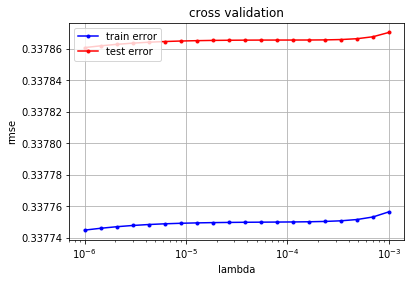
\includegraphics[scale=0.5]{linear_1}
\centering
\caption{MSE - Lambda plot for first degree linear model}
\end{figure}
\end{center}
\vspace{-15pt}
After testing the first degree linear model, we decided to add several degree polynomial basis to decrease bias and increase accuracy. The result plot is given below (Figure -2,3,4 and 5):
\begin{center}
\begin{figure}
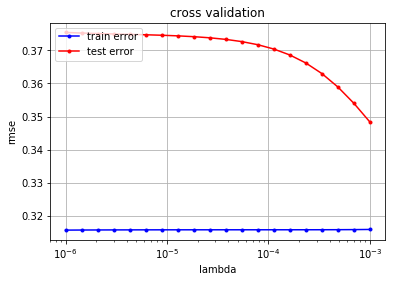
\includegraphics[scale=0.4]{linear_2}
\centering
\caption{MSE - Lambda plot for second degree linear model}
\textbf{\textcolor{red}{The best lambda value: 0.01, test error: 0.3483 and train error (for best test error): 0.3158}}
\vspace{5ex}

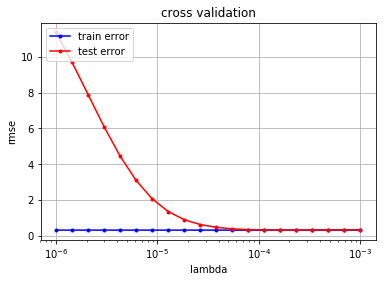
\includegraphics[scale=0.4]{linear_3}
\centering
\caption{MSE - Lambda plot for third degree linear model}
\textbf{\textcolor{red}{The best lambda value: 0.0001, test error: 0.306 and train error (for best test error): 0.304}}
\vspace{5ex}

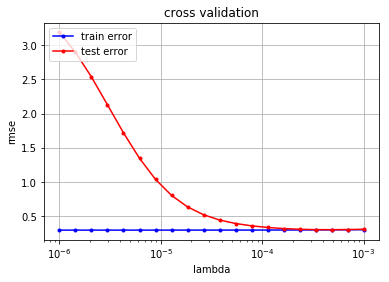
\includegraphics[scale=0.4]{linear_4}
\centering
\caption{MSE - Lambda plot for fourth degree linear model}
\textbf{\textcolor{red}{The best lambda value: 0.0004, test error: 0.303 and train error (for best test error): 0.301}}
\vspace{5ex}

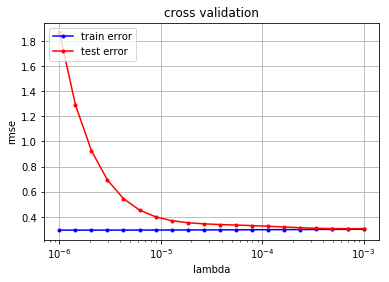
\includegraphics[scale=0.4]{linear_5}
\centering
\caption{MSE - Lambda plot for fifth degree linear model}
\textbf{\textcolor{red}{The best lambda value: 0.0006, test error: 0.305 and train error (for best test error): 0.301}}
\end{figure}
\end{center}
\newpage
As can be seen in the figures and results, while train error is continuously decreasing because of over-fitting, there is no significant change in test error after third degree polynomial basis. Therefore, feature extraction using polynomial basis does not seem working for higher degrees. Furthermore, the accuracy of the model in Kaggle is not as good as what we expected (0.79 - 0.8), so that we decided to switch logistic regression, which will be discussed in the next chapter, to enhance accuracy.
\section{Results}
Shows that accuracy is good enough meaning that model selection was good
\section{Discussion}
State that we can improve the accuracy by using non-linear classifiers?
\section{Summary}
We have shown that it is possible to detect the Higgs boson using linear methods and feature augmentation.

\begin{thebibliography}{99}
\bibitem{higgs} https://en.wikipedia.org/wiki/Higgs\_boson
\bibitem{data} REPLACE ME
\end{thebibliography}

\end{document}
